% Midterm report -- Math 129 final project
% Layout: if neurips_2025.sty / neurips_2024.sty is next to this file it is used
% (preprint mode); otherwise a plain article layout is used so the file still compiles.
% Figures and tables are generated by scripts/07_make_figures.py. Before compiling, copy
%   reports/figures  ->  figures/     and    reports/tables  ->  tables/
% next to this file (on Overleaf: upload both folders).
\documentclass[10pt]{article}
\usepackage{amsfonts,amsmath,amssymb,amsthm}% before the style: amsmath defines \And itself
\newif\ifnips
\IfFileExists{neurips_2025.sty}{\nipstrue\usepackage[preprint]{neurips_2025}}{%
\IfFileExists{neurips_2024.sty}{\nipstrue\usepackage[preprint]{neurips_2024}}{%
\usepackage[margin=1in]{geometry}}}
\ifnips\else\renewcommand{\And}{\and}\fi
\usepackage[utf8]{inputenc}
\usepackage[T1]{fontenc}
\usepackage{url}
\usepackage{booktabs}
\usepackage{microtype}
\usepackage{graphicx}
\usepackage{xcolor}
\usepackage[colorlinks=true,linkcolor=blue!50!black,citecolor=blue!50!black,urlcolor=blue!50!black]{hyperref}
\newtheorem{proposition}{Proposition}
\newtheorem{remark}{Remark}
\newcommand{\AUC}{\mathrm{AUC}}
\newcommand{\Prob}{\mathbb{P}}
\newcommand{\repourl}{https://github.com/YOUR-USERNAME/hbp_ln_math129_finalproject}% <-- edit

\title{Does Speech Carry Dementia and Parkinson's Signal Beyond Age and Recording Period?\\
A Confound-Aware Evaluation on EWA-DB}

\author{Hanna Parker \And [Partner name]\\
Math 129 --- Midterm report}

\IfFileExists{tables/numbers.tex}{% generated by 07_make_figures.py from reports/*.csv -- do not edit by hand
\newcommand{\adAddMeta}{+0.080}
\newcommand{\adAddMetaHi}{+0.109}
\newcommand{\adAddMetaLo}{+0.051}
\newcommand{\adAge}{0.841}
\newcommand{\adAgeHi}{0.865}
\newcommand{\adAgeLo}{0.813}
\newcommand{\adAllSpeech}{0.937}
\newcommand{\adCaliperAge}{0.592}
\newcommand{\adCondMax}{0.94}
\newcommand{\adCondMin}{0.90}
\newcommand{\adGap}{+0.273}
\newcommand{\adGapHi}{+0.338}
\newcommand{\adGapLo}{+0.203}
\newcommand{\adGapSeventy}{+0.307}
\newcommand{\adGapSeventyHi}{+0.391}
\newcommand{\adGapSeventyLo}{+0.219}
\newcommand{\adMatchAge}{0.622}
\newcommand{\adMatchCov}{126}
\newcommand{\adMatchPairs}{1{,}750}
\newcommand{\adMatchSpeech}{0.895}
\newcommand{\adMeta}{0.870}
\newcommand{\adMetaHi}{0.895}
\newcommand{\adMetaLo}{0.847}
\newcommand{\adMonthAge}{0.856}
\newcommand{\adMonthAgeHi}{+0.035}
\newcommand{\adMonthAgeLo}{$-$0.068}
\newcommand{\adMonthGap}{+0.013}
\newcommand{\adMonthGapHi}{+0.077}
\newcommand{\adMonthGapLo}{$-$0.047}
\newcommand{\adNPat}{149}
\newcommand{\adNaiveSE}{0.0006}
\newcommand{\adResAge}{+0.050}
\newcommand{\adResAgeHi}{+0.090}
\newcommand{\adResAgeLo}{+0.011}
\newcommand{\adSeventyCov}{114}
\newcommand{\adSeventyN}{135}
\newcommand{\adSpeech}{0.935}
\newcommand{\adSpeechHi}{0.956}
\newcommand{\adSpeechLo}{0.920}
\newcommand{\adSpeechMeta}{0.946}
\newcommand{\adSpeechMetaHi}{0.964}
\newcommand{\adSpeechMetaLo}{0.933}
\newcommand{\adSpeechMonth}{0.814}
\newcommand{\adSpeechMonthHi}{0.861}
\newcommand{\adSpeechMonthLo}{0.784}
\newcommand{\adSpeechRes}{0.883}
\newcommand{\adSpeechResHi}{0.914}
\newcommand{\adSpeechResLo}{0.864}
\newcommand{\adSpeechSE}{0.0092}
\newcommand{\adTAge}{0.932}
\newcommand{\adTAgeHi}{0.975}
\newcommand{\adTAgeLo}{0.877}
\newcommand{\adTMeta}{0.930}
\newcommand{\adTMetaHi}{0.980}
\newcommand{\adTMetaLo}{0.867}
\newcommand{\adTSpeech}{0.905}
\newcommand{\adTSpeechHi}{0.972}
\newcommand{\adTSpeechLo}{0.816}
\newcommand{\adTSpeechRes}{0.808}
\newcommand{\adTSpeechResHi}{0.908}
\newcommand{\adTSpeechResLo}{0.706}
\newcommand{\adTposTest}{32}
\newcommand{\batchAge}{0.42}
\newcommand{\batchDate}{0.38}
\newcommand{\batchLQ}{0.70}
\newcommand{\pdAddMeta}{+0.196}
\newcommand{\pdAddMetaHi}{+0.235}
\newcommand{\pdAddMetaLo}{+0.157}
\newcommand{\pdAge}{0.568}
\newcommand{\pdAgeHi}{0.612}
\newcommand{\pdAgeLo}{0.523}
\newcommand{\pdAllSpeech}{0.901}
\newcommand{\pdCaliperAge}{0.499}
\newcommand{\pdCondMax}{0.91}
\newcommand{\pdCondMin}{0.90}
\newcommand{\pdGap}{+0.415}
\newcommand{\pdGapHi}{+0.469}
\newcommand{\pdGapLo}{+0.357}
\newcommand{\pdGapSeventy}{+0.432}
\newcommand{\pdGapSeventyHi}{+0.544}
\newcommand{\pdGapSeventyLo}{+0.279}
\newcommand{\pdMatchAge}{0.497}
\newcommand{\pdMatchCov}{163}
\newcommand{\pdMatchPairs}{2{,}886}
\newcommand{\pdMatchSpeech}{0.912}
\newcommand{\pdMeta}{0.706}
\newcommand{\pdMetaHi}{0.751}
\newcommand{\pdMetaLo}{0.669}
\newcommand{\pdMonthAge}{+0.283}
\newcommand{\pdMonthAgeHi}{+0.337}
\newcommand{\pdMonthAgeLo}{+0.222}
\newcommand{\pdNPat}{175}
\newcommand{\pdResAge}{+0.314}
\newcommand{\pdResAgeHi}{+0.367}
\newcommand{\pdResAgeLo}{+0.259}
\newcommand{\pdSpeech}{0.895}
\newcommand{\pdSpeechHi}{0.927}
\newcommand{\pdSpeechLo}{0.875}
\newcommand{\pdSpeechMeta}{0.898}
\newcommand{\pdSpeechMetaHi}{0.929}
\newcommand{\pdSpeechMetaLo}{0.878}
\newcommand{\pdSpeechMonth}{0.840}
\newcommand{\pdSpeechMonthHi}{0.885}
\newcommand{\pdSpeechMonthLo}{0.814}
\newcommand{\pdSpeechRes}{0.872}
\newcommand{\pdSpeechResHi}{0.909}
\newcommand{\pdSpeechResLo}{0.849}
\newcommand{\pdTAge}{0.863}
\newcommand{\pdTAgeHi}{0.947}
\newcommand{\pdTAgeLo}{0.766}
\newcommand{\pdTMeta}{0.690}
\newcommand{\pdTMetaHi}{0.815}
\newcommand{\pdTMetaLo}{0.562}
\newcommand{\pdTSpeech}{0.690}
\newcommand{\pdTSpeechHi}{0.849}
\newcommand{\pdTSpeechLo}{0.541}
\newcommand{\pdTSpeechRes}{0.637}
\newcommand{\pdTSpeechResHi}{0.788}
\newcommand{\pdTSpeechResLo}{0.487}
\newcommand{\pdTposTest}{21}
\newcommand{\seRatio}{17}
}{\GenericError{}{Missing tables/numbers.tex}{Run scripts/07_make_figures.py and copy reports/tables and reports/figures next to main.tex}{}}
\begin{document}
\maketitle

\begin{abstract}
A recent preprint reports that deep spectrotemporal models detect dementia from Slovak speech. We re-examine this claim on the underlying database, EWA-DB, using 1,649 speakers and 112{,}846 recordings. First, the preprint's own confusion matrix shows its full model scoring 83.9\% accuracy against 95.1\% for a rule that always answers ``healthy'': it makes more false alarms than correct detections. Second, age alone separates Alzheimer's and mild cognitive impairment (AD/MCI) from healthy speakers at AUC $\adAge$, and recording period is also tied to diagnosis. We therefore evaluate precomputed acoustic features with participant-level splits, repeated cross-validation, speaker-level bootstrap intervals, and a \emph{conditional AUC} that scores only patient--control pairs recorded in the same month and at similar ages. We prove that this quantity is $1/2$ for any score that carries no information about the label beyond the matching variables. Speech reaches AUC $\adSpeech$ for AD/MCI and $\pdSpeech$ for Parkinson's disease (PD), and keeps $\adMatchSpeech$ and $\pdMatchSpeech$ in matched pairs, while age alone falls to $\adMatchAge$ and $\pdMatchAge$. However, speech also predicts recording date among healthy speakers ($R^2=\batchDate$), so we also train on early recordings and test on later ones. Site and device effects cannot be excluded with the released metadata.
\end{abstract}

%=====================================================================
\section{Introduction}
Speech is an attractive, non-invasive source of early markers for neurodegenerative disease, and several groups now publish models that report high accuracy. Small clinical datasets make such claims easy to get wrong: patients and controls differ in age, in how and when they were recruited, and in the circumstances of recording, and a model can profit from any of these without detecting disease.

We study EWA-DB, a Slovak speech database of healthy speakers and speakers with Alzheimer's disease (AD), mild cognitive impairment (MCI) and Parkinson's disease (PD) \cite{rusko2024}. A 2026 preprint by Ugwu and Oyeleke \cite{ugwu2026} proposes an ASR-agnostic CNN--ConvGRU model with a ``spectral dynamics'' branch and reports, for Slovak, accuracy $0.839$ and AUC $0.755$ for the full model and $0.937$ and $0.766$ for an audio-only ablation. We ask three questions.
\begin{enumerate}
\item[\textbf{Q1.}] Do the reported numbers show that the model detects disease?
\item[\textbf{Q2.}] How much of the diagnosis can be predicted without any speech, from age and recording metadata?
\item[\textbf{Q3.}] Does speech carry information beyond age and recording period, and does it generalise across time?
\end{enumerate}
\paragraph{Contributions.} (i) An audit of the preprint's Slovak result using accuracy, prevalence and precision (Section~\ref{sec:paper}). (ii) Quantified confounding in EWA-DB (Section~\ref{sec:data}). (iii) A confound-aware evaluation protocol with a short theory: a stratified AUC decomposition, a chance-level property of conditional AUC, an over-adjustment result for feature residualisation, and the U-statistic structure behind our bootstrap (Section~\ref{sec:theory}). (iv) Results for AD/MCI and PD with honest uncertainty (Section~\ref{sec:results}). We do not train deep audio models: only 44 AD/MCI speakers have released audio, and the database ships precomputed features for every speaker.

%=====================================================================
\section{Background}
\paragraph{EWA-DB.} The database holds recordings from 1,649 speakers made on mobile phones at 16\,kHz, each performing sustained phonation of /a/, a rapid /pa-ta-ka/ repetition (diadochokinesis), object and action naming, and picture description, with a clinical group, age, sex, education and a cognitive score (MoCA) per speaker. Only 1,003 speakers consented to audio release; features computed by the authors are provided for all \cite{rusko2024}. The license forbids redistribution, so our repository contains code and aggregate results only.

\paragraph{The preprint.} Ugwu and Oyeleke \cite{ugwu2026} merge AD and MCI, use stratified speaker-level 65/15/20\% splits, and train from 4-second log-Mel segments. Their Slovak ablation reports that a spectral-dynamics-only model reaches $0.951$ accuracy at AUC $0.506$, which they themselves attribute to majority-class prediction. We ask the same question of their full model.

\paragraph{Related work on EWA-DB.} La Quatra et al.\ \cite{laquatra2025} use EWA-DB for Parkinson's detection with a bilingual dual-head model. We do not reproduce their method; we use their task as a second, less confounded test case.

%=====================================================================
\section{Data and confounds}\label{sec:data}
\subsection{Speakers}
Table~\ref{tab:groups} summarises the groups. We exclude the two speakers with both AD and PD. Four speakers have impossible ages (for example 2022) and are treated as missing.

\begin{table}[t]
\centering\small
\begin{tabular}{lrrrr}
\toprule
Group & Speakers & With audio & Median age & Female\\
\midrule
Healthy (HC) & 1,323 & 863 & 65 & 71\%\\
AD & 87 & 41 & 80 & 72\%\\
MCI & 62 & 3 & 76.5 & 65\%\\
PD & 175 & 95 & 68 & 41\%\\
\bottomrule
\end{tabular}
\caption{EWA-DB speakers by clinical group (all 1,649 speakers have features; 1,003 have released audio).}
\label{tab:groups}
\end{table}

\subsection{Confounds}
\paragraph{Age.} No AD patient is under 60 and 45 of the 87 are over 79, whereas 407 of the 1,323 healthy speakers (31\%) are under 60. PD patients are close in age to controls.
\paragraph{Sex.} AD is as female as healthy controls (72\% versus 71\%), but PD is 59\% male.
\paragraph{Recording period.} Patients are recorded in clusters: 28 of the 87 AD patients were recorded in March 2023, against 5 of the 1,323 healthy controls. Recording month explains $19.9\%$ of the variance of the AD/MCI label ($28.4\%$ for AD, $8.8\%$ for PD); with 26 months, chance alone would explain about $1.7\%$.

\subsection{Features}
Each recording has a JSON file with 62 GeMAPS features, 28 NeuroSpeech features and a 2,048-dimensional Trill embedding (the README describes the toolkits). We use 109{,}839 recordings; 167 files (0.10--0.30\% of each group's files) lack a NeuroSpeech block and are skipped, and the two practice naming items are excluded. For each speaker and task (phonation, pataka, picture, naming) we average the GeMAPS and NeuroSpeech features over the task's recordings, giving $4\times 90$ features per speaker, and average the Trill embedding over all recordings, reduced to 32 dimensions by PCA. The JSON ``info'' block contains the diagnosis and is never read. The audio itself is not used.

\subsection{Splits}
Splits are participant-level, 65/15/20\% (train/validation/test), stratified by diagnosis and audio availability, with seed 42; the split is identified by a hash of the speaker-to-split assignment (prefix \texttt{490941a1}). The AD/MCI test set contains only 30 patients and the PD test set 35, so we complement the fixed split with repeated cross-validation over all speakers.

%=====================================================================
\section{Methods}\label{sec:methods}
\paragraph{Classifier.} $\ell_2$-regularised logistic regression with balanced class weights and a fixed $C=0.01$ (chosen in advance, not tuned on any evaluation data). Median imputation, standardisation, PCA and residualisation are fitted on training data only, inside every fold.

\paragraph{Feature sets.} \emph{Age only}; \emph{all metadata} (age, sex, education years, recording date, quality flag); \emph{speech} (GeMAPS, NeuroSpeech and Trill); \emph{speech + all metadata}; \emph{speech (age/sex removed)}, where each feature has its linear prediction from age and sex subtracted; and \emph{speech (age/sex/month removed)}, which also removes recording-month indicators.

\paragraph{Cross-validation.} Out-of-fold scores come from $5\times5$-fold stratified cross-validation over all speakers in a comparison (149 AD/MCI and 1,323 healthy; 175 PD and 1,323 healthy). Each speaker's scores are averaged over the five repeats before computing AUC.

\paragraph{Uncertainty.} Intervals are 95\% bootstrap percentile intervals from resampling \emph{speakers} (1000 resamples; 500 for conditional AUC). Paired differences use the same resamples for both models. We treat the out-of-fold scores as fixed, so the intervals do not include training-set variability and are somewhat optimistic.

\paragraph{Conditional AUC.} For a set of patient--control pairs allowed by a condition (same calendar month, same 14-day window, age within 5 years, or the last two combined), conditional AUC is the share of allowed pairs in which the patient scores higher, counting ties as one half. Section~\ref{sec:theory} gives its meaning. We evaluate the same fixed out-of-fold scores, so no model is retrained.

\paragraph{Other checks.} \emph{Batch predictability:} among healthy speakers only, can speech predict age, recording date (ridge regression, $R^2$) or the low-quality flag (AUC)? \emph{Temporal split:} train on speakers recorded before 2023-01-01, test on speakers recorded on or after it.

%=====================================================================
\section{Theory}\label{sec:theory}
Let $Y\in\{0,1\}$ be the label and $S$ a real score. Draw $(S_1,Z_1)$ from the law of $(S,Z)$ given $Y=1$ and, independently, $(S_0,Z_0)$ given $Y=0$, where $Z$ is any variable we want to control for (recording month, an age band). The AUC is
\[
\AUC=\Prob(S_1>S_0)+\tfrac12\Prob(S_1=S_0)
\]
(Hanley and McNeil \cite{hanley1982}): the chance that a random patient outscores a random control.

\subsection{Accuracy, prevalence and precision}\label{sec:acc}
\begin{proposition}\label{prop:acc}
For a classifier with $TP$, $FP$ true and false positives on $N$ speakers, accuracy $=(1-\pi)+(TP-FP)/N$, where $\pi$ is the prevalence. It therefore beats the rule ``always predict healthy'' if and only if $TP>FP$, that is, precision $>1/2$.
\end{proposition}
\begin{proof}
Accuracy is $(TN+TP)/N$ and $TN=N(1-\pi)-FP$, since there are $N(1-\pi)$ healthy speakers. The always-healthy rule has accuracy $1-\pi$. \qedhere
\end{proof}
In contrast, the AUC depends only on the two class-conditional score distributions, not on $\pi$.

\subsection{A stratified decomposition and a chance-level property}
\begin{proposition}[Decomposition]\label{prop:decomp}
For any event $E$ in $(Z_1,Z_0)$ with $0<\Prob(E)<1$,
\[
\AUC=\Prob(E)\,\AUC_E+\bigl(1-\Prob(E)\bigr)\,\AUC_{E^c},
\]
where $\AUC_E=\Prob(S_1>S_0\mid E)+\tfrac12\Prob(S_1=S_0\mid E)$ and likewise for $E^c$.
\end{proposition}
This is the law of total probability.

\begin{proposition}[Chance level within strata]\label{prop:chance}
Let $Z$ be discrete and $E=\{Z_1=Z_0\}$ with $\Prob(E)>0$. If $S\perp Y\mid Z$ (the score carries no information about the label beyond $Z$), then $\AUC_E=1/2$.
\end{proposition}
\begin{proof}
Let $p_y(z)=\Prob(Z=z\mid Y=y)$. Conditional on $Z_1=Z_0=z$, the scores $S_1,S_0$ are independent draws from the same law $\mathcal L(S\mid Z=z)$, because $S\perp Y\mid Z$. For two i.i.d.\ draws $\Prob(S_1>S_0)=\Prob(S_0>S_1)$, so $\Prob(S_1>S_0\mid z)+\tfrac12\Prob(S_1=S_0\mid z)=\tfrac12$. Conditional on $E$, the stratum $z$ has probability $p_1(z)p_0(z)/\Prob(E)$; averaging gives $\AUC_E=\tfrac12$. \qedhere
\end{proof}
Hence an observed $\AUC_E>1/2$ is evidence against the null $S\perp Y\mid Z$: the score separates patients from controls \emph{within} strata. Conversely, the overall AUC can exceed $1/2$ with the null true.

\begin{proposition}[Stratum detector]\label{prop:detector}
Let $Z\in\{a,b\}$, $q_y=\Prob(Z=b\mid Y=y)$, and $S=\mathbf 1[Z=b]$. Then $\AUC=\tfrac12+\tfrac12(q_1-q_0)$, while $\AUC_{\{Z_1=Z_0\}}=1/2$.
\end{proposition}
\begin{proof}
$\AUC=q_1(1-q_0)+\tfrac12\bigl[q_1q_0+(1-q_1)(1-q_0)\bigr]=\tfrac12+\tfrac12(q_1-q_0)$. Within a stratum $S_1=S_0$, so every pair is a tie. \qedhere
\end{proof}
\begin{remark}
In EWA-DB, $q_1=28/87=0.322$ for AD and $q_0=5/1323=0.004$ for healthy speakers for the stratum ``recorded in March 2023''. A detector with no speech information therefore achieves AUC $=0.66$ for AD versus healthy.
\end{remark}
For continuous strata such as age, a caliper (age within 5 years) is only an approximate stratum, so an age-only score keeps some residual advantage inside the caliper; we see $\adCaliperAge$ rather than $0.50$ for AD/MCI.

\subsection{Why removing recording month over-adjusts}
\begin{proposition}[Over-adjustment]\label{prop:overadj}
Suppose features follow $V=\beta Y+\Gamma M+\varepsilon$ where $M$ is a one-hot month vector, $\varepsilon$ has mean zero and is independent of $(Y,M)$. Regressing $V$ on $M$ leaves the residual $R=\beta\,(Y-\mathbb E[Y\mid M])+\varepsilon$, so the label signal in $R$ has variance $\beta\beta^\top\,\mathbb E[\mathrm{Var}(Y\mid M)]$, a fraction $1-R^2_{Y\sim M}$ of the unadjusted signal $\beta\beta^\top\pi(1-\pi)$.
\end{proposition}
\begin{proof}
$\mathbb E[V\mid M]=\beta\,\mathbb E[Y\mid M]+\Gamma M$, so subtracting it gives the stated $R$. The law of total variance, $\mathrm{Var}(Y)=\mathbb E[\mathrm{Var}(Y\mid M)]+\mathrm{Var}(\mathbb E[Y\mid M])$, and $R^2_{Y\sim M}=\mathrm{Var}(\mathbb E[Y\mid M])/\mathrm{Var}(Y)$ give the fraction. \qedhere
\end{proof}
Because patients cluster in a few months, $R^2_{Y\sim M}=0.20$ for AD/MCI in our data: removing month from the \emph{features} discards a fifth of the label variance even when the month has no causal link to speech. Conditional AUC avoids this: the classifier is trained on all information, and month only restricts which pairs we use to \emph{score} it.

\subsection{Uncertainty: why we resample speakers}
For a fixed score function and $n_1$ patients and $n_0$ controls, $\hat U=\frac1{n_1n_0}\sum_{i,j}\bigl[\mathbf 1(s_i>s_j)+\tfrac12\mathbf 1(s_i=s_j)\bigr]$ is a two-sample U-statistic of Hoeffding \cite{hoeffding1948}. Writing $V_{10}(s)=\Prob(S_0<s)+\tfrac12\Prob(S_0=s)$ and $V_{01}(s)=\Prob(S_1>s)+\tfrac12\Prob(S_1=s)$,
\[
\mathrm{Var}(\hat U)=\frac{\sigma_{10}^2}{n_1}+\frac{\sigma_{01}^2}{n_0}+O\!\Bigl(\frac1{n_1n_0}\Bigr),\quad \sigma_{10}^2=\mathrm{Var}\,V_{10}(S_1),\ \sigma_{01}^2=\mathrm{Var}\,V_{01}(S_0)
\]
(DeLong et al.\ \cite{delong1988}). The variance is governed by the number of \emph{speakers}, not pairs: each speaker appears in many pairs and the pairs are dependent. Treating our 197{,}127 AD/MCI--healthy pairs as independent would give a standard error near $\adNaiveSE$ at AUC $\adSpeech$; the bootstrap over speakers gives about $\adSpeechSE$, roughly $\seRatio$ times larger. For conditional AUC we resample speakers with multiplicity counts and give each pair the product of its two speakers' counts.

%=====================================================================
\section{Results}\label{sec:results}
\subsection{The preprint's Slovak result}\label{sec:paper}
Figure~\ref{fig:paper} reads the confusion matrix in the preprint's Figure~1(b) for the Slovak full model: $TN=735$, $FP=128$, $FN=18$, $TP=26$, so $N=907$ with 44 AD/MCI speakers. The accuracy is $0.839$, matching their Table~2, but always answering ``healthy'' gives $863/907=0.951$. Proposition~\ref{prop:acc} makes this transparent: accuracy minus the baseline is $(26-128)/907=-0.113$. Sensitivity is $59\%$, specificity $85\%$ and the precision for AD/MCI is $26/154=17\%$. The $0.937$ precision in their Table~2 equals the class-weighted average of the two classes' precision computed from this matrix, which is dominated by the healthy class; their ``recall'' of $0.839$ equals their accuracy, as weighted recall does.

The size of the matrix is also informative: $907=863+41+3$ is exactly the number of healthy, AD and MCI speakers with released audio in EWA-DB. That is consistent with evaluation on every such speaker rather than a held-out 20\% (about 200), which would affect the interpretation of their numbers. We flag this as an inference and not a finding; it is a question for the authors.

\begin{figure}[t]
\centering
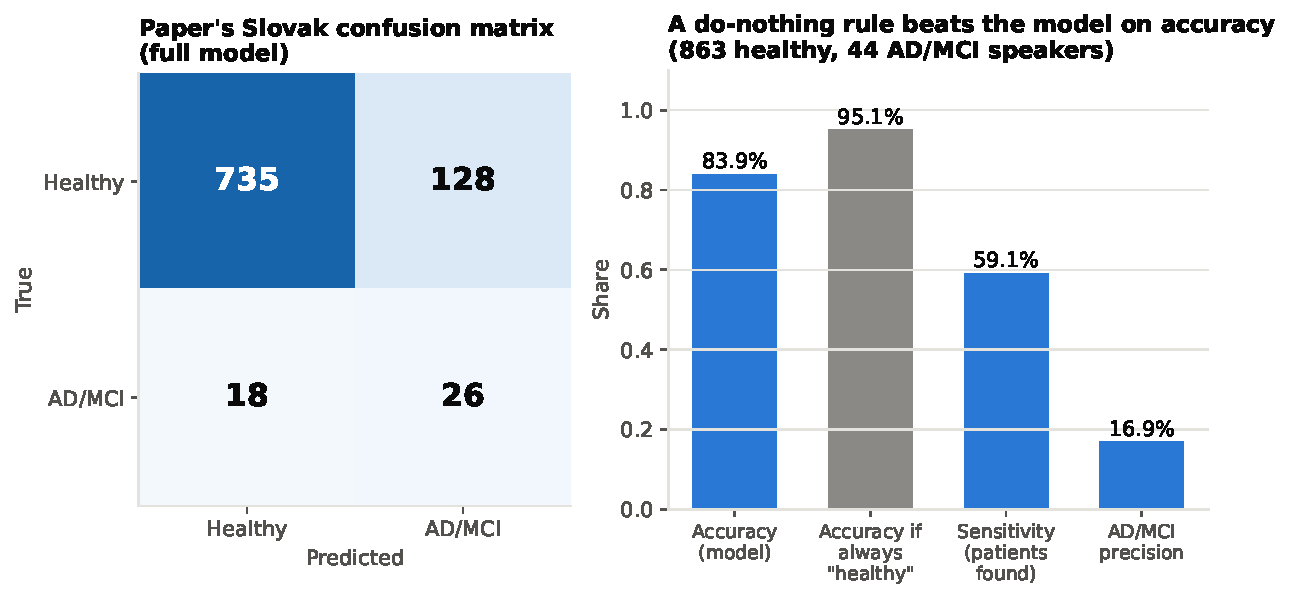
\includegraphics[width=\linewidth]{figures/fig1_paper_critique.pdf}
\caption{The preprint's Slovak full-model confusion matrix (read from its Figure~1(b)) and metrics. Always predicting ``healthy'' beats the model's accuracy; AD/MCI precision is $17\%$.}
\label{fig:paper}
\end{figure}

\subsection{Metadata alone predicts diagnosis}
Figure~\ref{fig:baselines} and Table~\ref{tab:cv_auc} give out-of-fold AUCs. For AD/MCI versus healthy, age alone reaches $\adAge$ (95\% CI $\adAgeLo$--$\adAgeHi$) and all metadata $\adMeta$ ($\adMetaLo$--$\adMetaHi$); the preprint's best Slovak AUC is $0.766$. This comparison is not like for like (our population, protocol and evaluation unit differ), but it shows that a no-speech benchmark already exceeds their reported discrimination. For PD, age alone gives $\pdAge$ and all metadata $\pdMeta$: PD is much less confounded by age.

\subsection{Speech adds signal beyond metadata}
Speech reaches AUC $\adSpeech$ ($\adSpeechLo$--$\adSpeechHi$) for AD/MCI and $\pdSpeech$ ($\pdSpeechLo$--$\pdSpeechHi$) for PD. Table~\ref{tab:paired} gives paired differences. Adding speech to all metadata improves AUC by $\adAddMeta$ ($\adAddMetaLo$ to $\adAddMetaHi$) for AD/MCI and $\pdAddMeta$ ($\pdAddMetaLo$ to $\pdAddMetaHi$) for PD. With age and sex linearly removed, speech still beats age alone by $\adResAge$ ($\adResAgeLo$ to $\adResAgeHi$) for AD/MCI and $\pdResAge$ ($\pdResAgeLo$ to $\pdResAgeHi$) for PD. Also removing recording month brings AD/MCI speech to $\adSpeechMonth$ ($\adSpeechMonthLo$--$\adSpeechMonthHi$), a difference from age alone of $\adMonthAge$ ($\adMonthAgeLo$ to $\adMonthAgeHi$), and PD speech to $\pdSpeechMonth$. By Proposition~\ref{prop:overadj} this removal discards part of the disease signal as well, so it is a lower bound, not a clean estimate.

\paragraph{A note on the single split.} On the fixed test split, speech plus age, sex and education beat age, sex and education alone by $0.046$ for AD/MCI with interval $-0.010$ to $0.097$ (30 test patients): inconclusive. With all 149 patients in cross-validation the interval is much tighter, which is why we report cross-validation.

\begin{figure}[t]
\centering
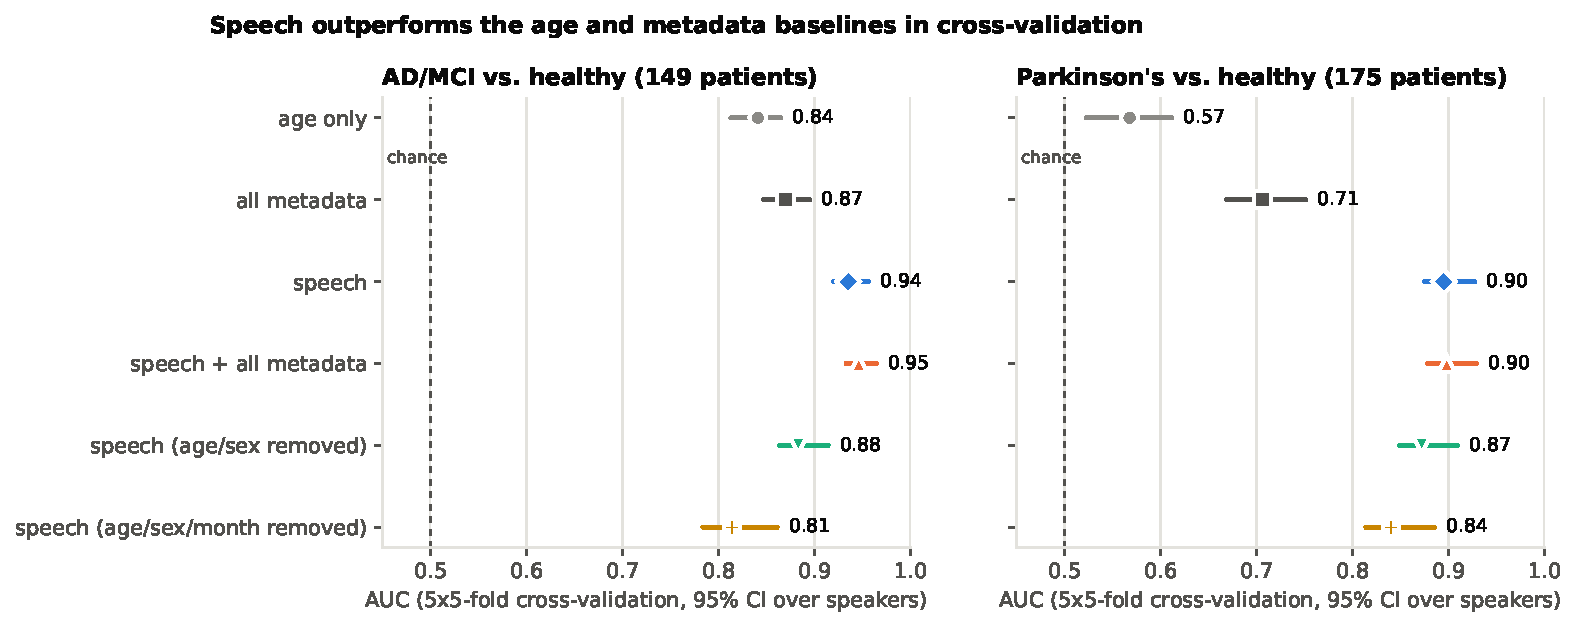
\includegraphics[width=\linewidth]{figures/fig2_baselines.pdf}
\caption{Out-of-fold AUC with 95\% CIs (speaker bootstrap) for each feature set.}
\label{fig:baselines}
\end{figure}

\begin{table}[t]
\centering
\small
\resizebox{\linewidth}{!}{%
\begin{tabular}{llrcrc}
\toprule
Task & Features & AUC & 95\% CI & AUC (70+) & 95\% CI (70+) \\
\midrule
AD/MCI vs. healthy & age only & 0.841 & [0.81, 0.86] & 0.633 & [0.58, 0.69] \\
 & all metadata & 0.870 & [0.85, 0.90] & 0.728 & [0.68, 0.77] \\
 & speech & 0.935 & [0.92, 0.96] & 0.906 & [0.87, 0.93] \\
 & speech + all metadata & 0.946 & [0.93, 0.96] & 0.919 & [0.89, 0.94] \\
 & speech (age/sex removed) & 0.883 & [0.86, 0.91] & 0.903 & [0.87, 0.93] \\
 & speech (age/sex/month removed) & 0.814 & [0.78, 0.86] & 0.841 & [0.80, 0.88] \\
Parkinson's vs. healthy & age only & 0.568 & [0.52, 0.61] & 0.475 & [0.40, 0.55] \\
 & all metadata & 0.706 & [0.67, 0.75] & 0.720 & [0.66, 0.78] \\
 & speech & 0.895 & [0.88, 0.93] & 0.892 & [0.84, 0.93] \\
 & speech + all metadata & 0.898 & [0.88, 0.93] & 0.903 & [0.86, 0.94] \\
 & speech (age/sex removed) & 0.872 & [0.85, 0.91] & 0.885 & [0.84, 0.93] \\
 & speech (age/sex/month removed) & 0.840 & [0.81, 0.89] & 0.859 & [0.80, 0.91] \\
\bottomrule
\end{tabular}}
\caption{Out-of-fold AUC from 5x5-fold cross-validation over all speakers. Bootstrap CIs resample speakers.}
\label{tab:cv_auc}
\end{table}

\begin{table}[t]
\centering
\small
\resizebox{\linewidth}{!}{%
\begin{tabular}{lllrcc}
\toprule
Task & Candidate & Reference & AUC diff. & 95\% CI & CI excl. 0 \\
\midrule
AD/MCI vs. healthy & speech + all metadata & all metadata & +0.080 & [0.05, 0.11] & yes \\
AD/MCI vs. healthy & speech (age/sex removed) & age only & +0.050 & [0.01, 0.09] & yes \\
AD/MCI vs. healthy & speech (age/sex/month removed) & age only & -0.017 & [-0.07, 0.04] & no \\
AD/MCI vs. healthy (70+) & speech (age/sex removed) & age only & +0.270 & [0.21, 0.33] & yes \\
AD/MCI vs. healthy (70+) & speech (age/sex/month removed) & age only & +0.208 & [0.14, 0.28] & yes \\
Parkinson's vs. healthy & speech + all metadata & all metadata & +0.196 & [0.16, 0.23] & yes \\
Parkinson's vs. healthy & speech (age/sex removed) & age only & +0.314 & [0.26, 0.37] & yes \\
Parkinson's vs. healthy & speech (age/sex/month removed) & age only & +0.283 & [0.22, 0.34] & yes \\
Parkinson's vs. healthy (70+) & speech (age/sex removed) & age only & +0.410 & [0.32, 0.49] & yes \\
Parkinson's vs. healthy (70+) & speech (age/sex/month removed) & age only & +0.384 & [0.28, 0.48] & yes \\
\bottomrule
\end{tabular}}
\caption{Paired AUC differences on the same out-of-fold scores (bootstrap over speakers).}
\label{tab:paired}
\end{table}


\subsection{Does the signal survive matching?}
Figure~\ref{fig:matched} and Table~\ref{tab:matched} evaluate the same scores on restricted pairs. For AD/MCI, speech scores $\adAllSpeech$ over all pairs and $\adMatchSpeech$ when patient and control share a recording month and differ in age by at most 5 years ($\adMatchPairs$ pairs; $\adMatchCov$ of the $\adNPat$ patients have a match); age alone falls from $\adAge$ to $\adMatchAge$. The gap between speech and age alone is $\adGap$ ($\adGapLo$ to $\adGapHi$). For speakers aged 70 and over it is $\adGapSeventy$ ($\adGapSeventyLo$ to $\adGapSeventyHi$; $\adSeventyCov$ of $\adSeventyN$ patients matched). For PD, speech ranges from $\pdCondMin$ to $\pdCondMax$ across conditions ($\pdMatchSpeech$ matched) while age alone is $\pdMatchAge$ (gap $\pdGap$; $\pdGapLo$ to $\pdGapHi$).

Two cautions. First, within age-matched pairs, age carries little information by construction, so beating age is partly built in; the more informative fact is that speech AUC barely moves across conditions. Second, within a month and \emph{without} age matching, age alone is still strong ($\adMonthAge$ for AD/MCI) and speech with age and sex removed differs from it by $\adMonthGap$ ($\adMonthGapLo$ to $\adMonthGapHi$). By Proposition~\ref{prop:chance}, a high speech AUC in matched pairs is evidence against a score that only tracks age and month, but month is a coarse proxy for a recording session.

\begin{figure}[t]
\centering
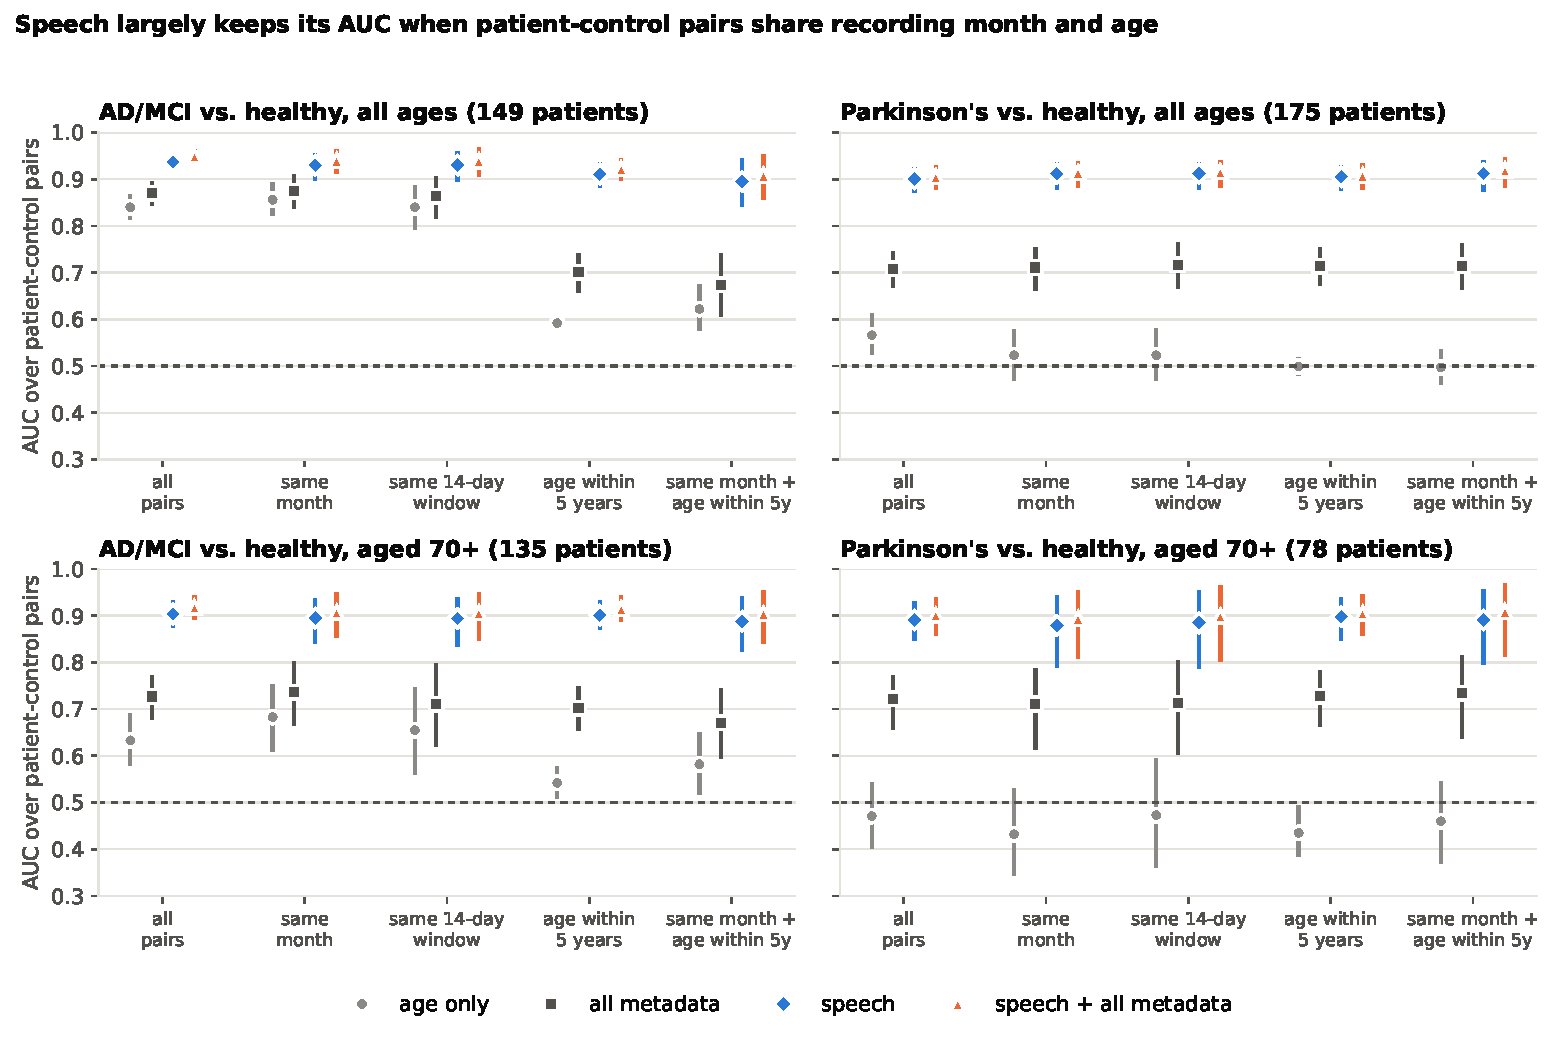
\includegraphics[width=\linewidth]{figures/fig3_matched_pairs.pdf}
\caption{Conditional AUC under increasingly strict pairing. Dashed line: chance.}
\label{fig:matched}
\end{figure}
\begin{table}[t]
\centering
\small
\resizebox{\linewidth}{!}{%
\begin{tabular}{lllrrrr}
\toprule
Task & Pairs & \#pairs & age only & all metadata & speech & speech + all metadata \\
\midrule
AD/MCI vs. healthy & all pairs & 197,127 & 0.840 [0.81, 0.87] & 0.870 [0.84, 0.90] & 0.937 [0.92, 0.95] & 0.949 [0.93, 0.96] \\
AD/MCI vs. healthy & same month + age within 5y & 1,750 & 0.622 [0.58, 0.68] & 0.674 [0.61, 0.74] & 0.895 [0.84, 0.94] & 0.908 [0.86, 0.95] \\
Parkinson's vs. healthy & all pairs & 231,525 & 0.566 [0.52, 0.61] & 0.708 [0.67, 0.74] & 0.901 [0.87, 0.93] & 0.905 [0.88, 0.93] \\
Parkinson's vs. healthy & same month + age within 5y & 2,886 & 0.497 [0.46, 0.54] & 0.715 [0.66, 0.76] & 0.912 [0.87, 0.94] & 0.919 [0.88, 0.95] \\
\bottomrule
\end{tabular}}
\caption{Conditional AUC: the share of patient-control pairs, restricted as shown, in which the patient scores higher. Brackets: 95\% bootstrap CI over speakers.}
\label{tab:matched}
\end{table}


\subsection{Speech encodes the recording period}
Among healthy speakers only, so that disease cannot drive the result, speech features predict recording date with $R^2=\batchDate$, age with $R^2=\batchAge$, and the low-quality flag with AUC $\batchLQ$ (Table~\ref{tab:batch}). The features therefore carry information about when a person was recorded, which is the route by which batch effects can leak into a classifier.
\begin{table}[t]
\centering
\small
\resizebox{\linewidth}{!}{%
\begin{tabular}{lrr}
\toprule
Predicted from speech & Healthy speakers & Score \\
\midrule
age ($R^2$) & 1321 & 0.42 \\
recording date ($R^2$) & 1323 & 0.38 \\
LOW\_QUALITY flag (AUC) & 1323 & 0.70 \\
\bottomrule
\end{tabular}}
\caption{Can speech features predict recording circumstances? Healthy speakers only, 5-fold CV. R$^2$ of 0 and AUC of 0.5 mean no information.}
\label{tab:batch}
\end{table}


\subsection{Generalisation across time}
Training on speakers recorded before 2023 and testing on later ones (Figure~\ref{fig:temporal}, Table~\ref{tab:temporal}), speech for PD scores $\pdTSpeech$ ($\pdTSpeechLo$--$\pdTSpeechHi$, $\pdTposTest$ test patients) against a cross-validation value of $\pdSpeech$, and speech with age and sex removed gives $\pdTSpeechRes$. For AD/MCI ($\adTposTest$ test patients) speech scores $\adTSpeech$ against $\adTAge$ for age alone. These test sets are small and the late-period population differs, so we treat the result as exploratory.
\begin{figure}[t]
\centering
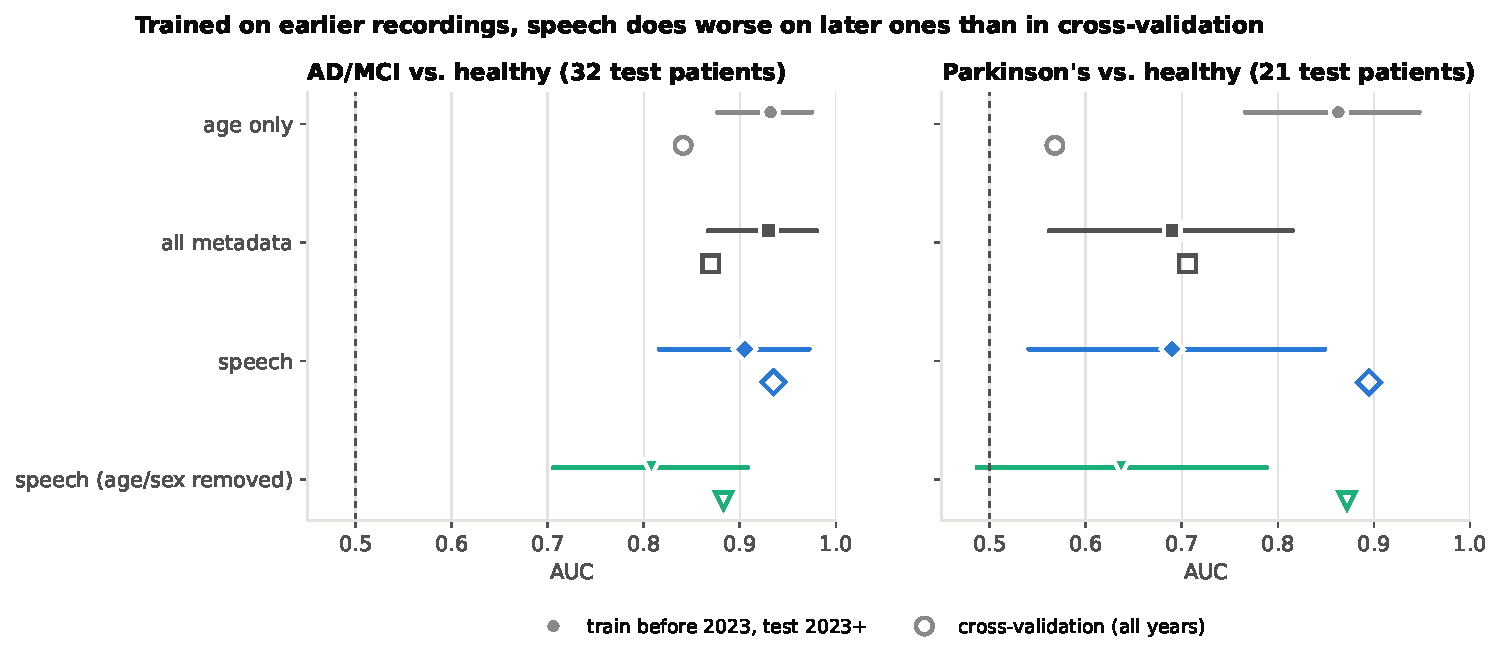
\includegraphics[width=\linewidth]{figures/fig4_temporal.pdf}
\caption{Temporal split (filled, with 95\% CI) versus cross-validation (open).}
\label{fig:temporal}
\end{figure}
\begin{table}[t]
\centering
\small
\resizebox{\linewidth}{!}{%
\begin{tabular}{llrrc}
\toprule
Task & Features & Pos. train/test & AUC & 95\% CI \\
\midrule
AD/MCI vs. healthy & age only & 117/32 & 0.932 & [0.88, 0.97] \\
AD/MCI vs. healthy & all metadata & 117/32 & 0.930 & [0.87, 0.98] \\
AD/MCI vs. healthy & speech & 117/32 & 0.905 & [0.82, 0.97] \\
AD/MCI vs. healthy & speech (age/sex removed) & 117/32 & 0.808 & [0.71, 0.91] \\
Parkinson's vs. healthy & age only & 154/21 & 0.863 & [0.77, 0.95] \\
Parkinson's vs. healthy & all metadata & 154/21 & 0.690 & [0.56, 0.81] \\
Parkinson's vs. healthy & speech & 154/21 & 0.690 & [0.54, 0.85] \\
Parkinson's vs. healthy & speech (age/sex removed) & 154/21 & 0.637 & [0.49, 0.79] \\
\bottomrule
\end{tabular}}
\caption{Train on speakers recorded before 2023-01-01, test on speakers recorded on or after it. Small test sets: treat as exploratory.}
\label{tab:temporal}
\end{table}


%=====================================================================
\section{Discussion and limitations}
\paragraph{What we can say.} (1) The preprint's headline Slovak accuracy is below the majority-class baseline and its AD/MCI precision is $17\%$. (2) In EWA-DB, age, sex, education and recording date alone predict AD/MCI at AUC $\adMeta$. (3) Precomputed speech features carry signal beyond these, with the strongest case for PD and for AD/MCI among older speakers, and the signal remains in age- and month-matched pairs.

\paragraph{What we cannot say.}
\begin{itemize}
\item \emph{Site and device.} Patients and controls were recruited at different places, and device, room and administrator can differ even within a month. The released metadata contain no such field, so our matching cannot rule this out; the batch-predictability result is consistent with a residual dependence.
\item \emph{Generalisation.} Results come from one Slovak database and a few hundred patients. The temporal split uses $\pdTposTest$ PD and $\adTposTest$ AD/MCI test patients.
\item \emph{Comparison to the preprint.} Our protocol (cross-validation over all speakers, precomputed features, logistic regression) differs from theirs, so we do not claim to have reproduced or refuted their AUC, only to have shown that simple baselines are strong and that their accuracy is not informative.
\item \emph{Method limits.} Residualisation is linear; the bootstrap treats out-of-fold scores as fixed; month is a coarse proxy; we ran many comparisons without correction, so isolated intervals that exclude zero should not be over-read.
\item \emph{Audio models.} We did not run deep models on raw audio; only 44 AD/MCI speakers have released audio.
\end{itemize}

\paragraph{Next steps.} A within-stratum permutation test (labels permuted within month and age band), which is exact under $S\perp Y\mid Z$ for exchangeable data; a same-day condition to measure how often patients and controls share sessions; and requesting the preprint authors' split lists and metric conventions.

%=====================================================================
\section{Conclusion}
Speech features distinguish AD/MCI and PD patients from healthy speakers in EWA-DB beyond what age and recording metadata explain, and the signal largely survives matching on recording month and age. But the same features encode the recording period, the temporal split is small and exploratory, and the preprint's reported accuracy does not exceed the do-nothing baseline. Credible evidence for speech-based screening in this database requires evaluation that controls for age and session, and honest intervals.

\paragraph{Reproducibility.} Code and aggregate results: \url{\repourl}. Scripts 01--07 reproduce every number from the released database (splits seed 42, fingerprint prefix \texttt{490941a1}). The data themselves cannot be redistributed.

\paragraph{AI assistance.} % Edit to match the course's disclosure policy.
Claude (Anthropic) assisted with experimental design, code and drafting. The authors ran all code on their own machines and are responsible for the content.

\begin{thebibliography}{9}\small
\bibitem{rusko2024} M.~Rusko et al. Slovak database of speech affected by neurodegenerative diseases. \emph{Scientific Data}, 2024.
\bibitem{ugwu2026} Ugwu and Oyeleke. ASR-agnostic multimodal spectrotemporal modeling for early dementia detection. arXiv:2606.30646, 2026.
\bibitem{laquatra2025} M.~La Quatra et al. Bilingual dual-head deep model for Parkinson's disease detection from speech. \emph{ICASSP}, 2025.
\bibitem{hanley1982} J.~A. Hanley and B.~J. McNeil. The meaning and use of the area under a receiver operating characteristic (ROC) curve. \emph{Radiology}, 143(1):29--36, 1982.
\bibitem{delong1988} E.~R. DeLong, D.~M. DeLong, and D.~L. Clarke-Pearson. Comparing the areas under two or more correlated receiver operating characteristic curves: a nonparametric approach. \emph{Biometrics}, 44(3):837--845, 1988.
\bibitem{hoeffding1948} W.~Hoeffding. A class of statistics with asymptotically normal distribution. \emph{Annals of Mathematical Statistics}, 19(3):293--325, 1948.
\end{thebibliography}

\end{document}
